\section{Application Design}
\label{sec:app}

In this section, we introduces the basic functions of our application and the design of it.


\subsection{Functions}
\label{sec:func}
The purpose of this application is to interactively visualize word co-occurrence networks and collecting feedbacks from user. Therefore, the application should have these basic functions:

\begin{enumerate}
	\item Pass questions and network information from back-end program to the front-end interface.
	\item User interface functions:
	\begin{enumerate}
		\item Display the questions and answers.
		\item Support selection behavior, and return the user selections.
		\item Display the visualization of word networks of user selected words
		\end{enumerate}
		
	\item Pass user feedbacks to the back-end and generate new data based on user feedbacks.
\end{enumerate}


\subsection{User Interface Design}


To include the functions we describe in Section \ref{sec:func}, we divide the major part of the user interface into two parts, the questions area and the visualization area.

\subsubsection{Overall Interface}

Figure \ref{fig:net_demo} shows the overall design of our interface. 

\begin{figure}[h]
\centering
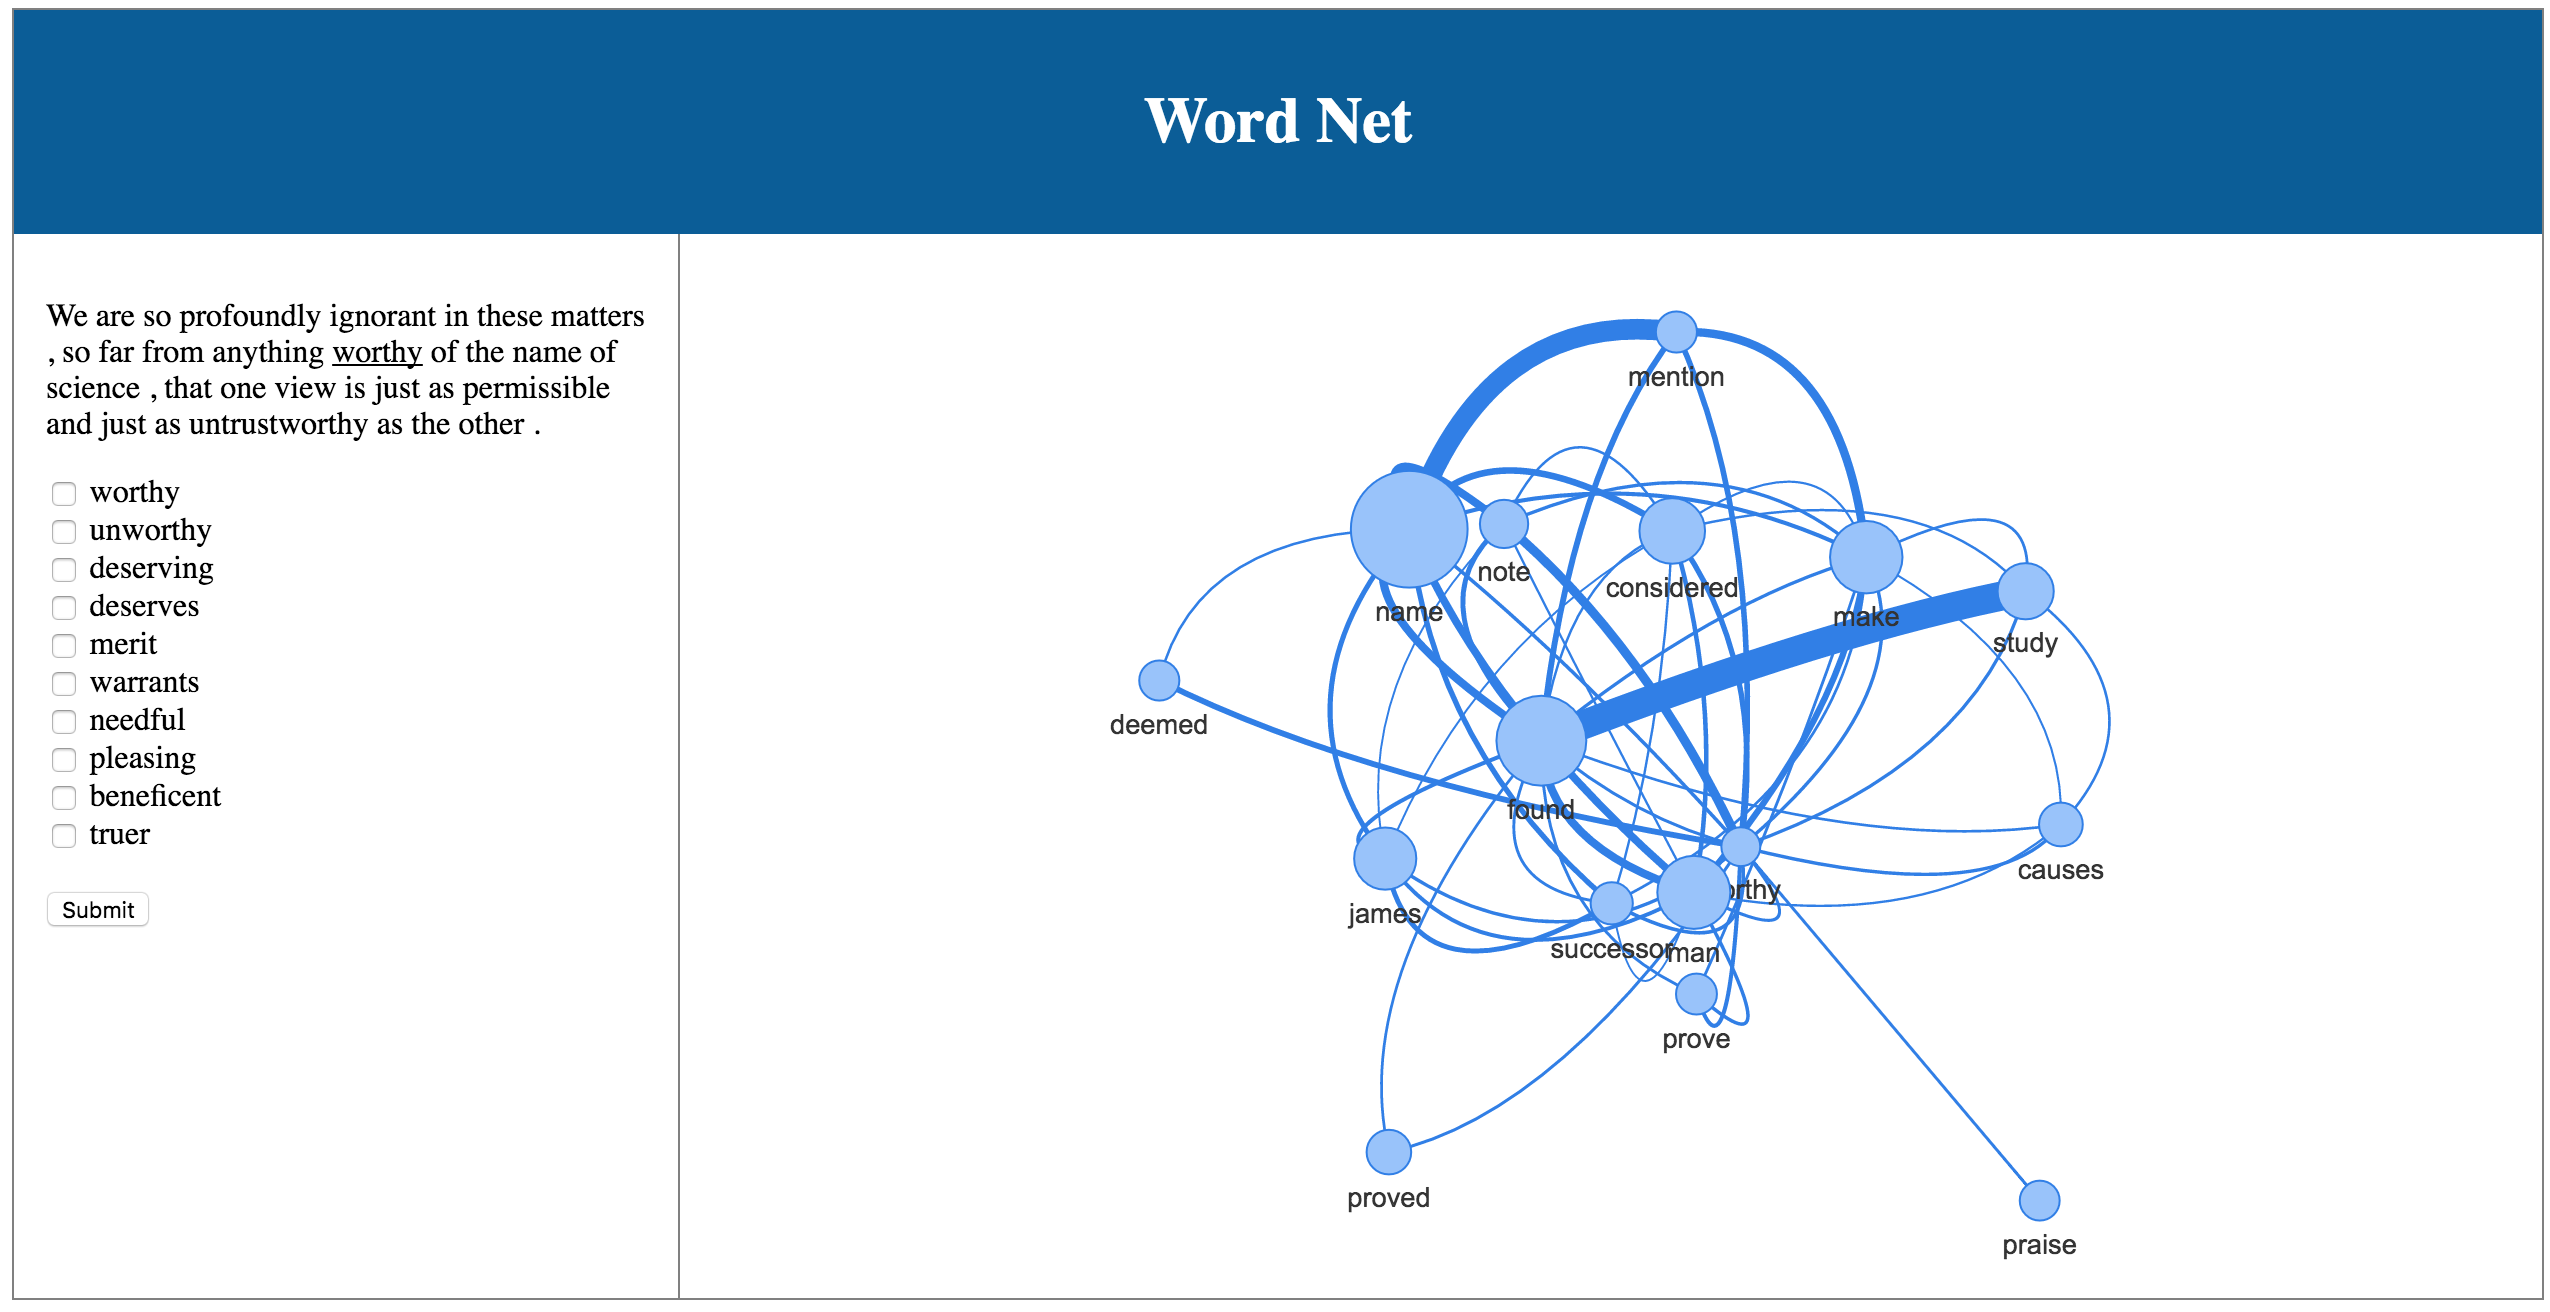
\includegraphics[width=0.95\linewidth]{figure/net_demo}
\caption{Demonstration of the overall user interface for interactively word network visualization}
\label{fig:net_demo}
\end{figure}


\subsubsection{Question Area}

The question area on left in Figure \ref{fig:net_demo} is the major area that user can make interactions, including making selections, picking one word to visualize the network and submitting their feedbacks. 

\begin{figure}[h]
\centering
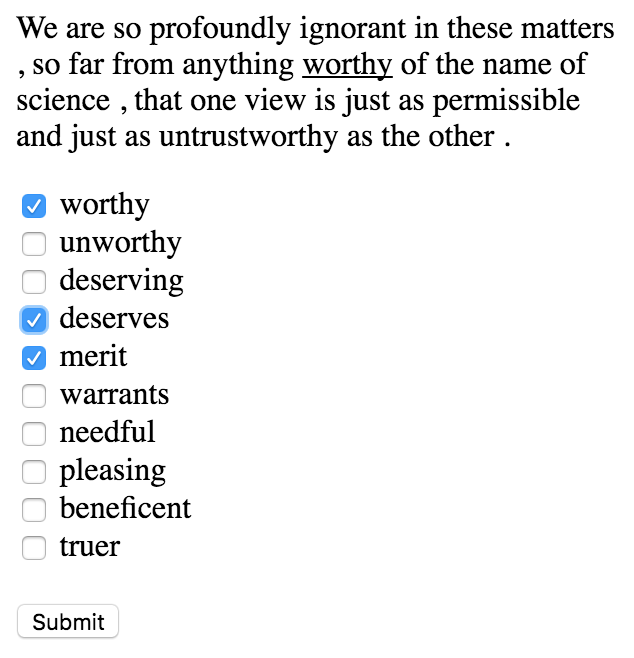
\includegraphics[width=0.8\linewidth]{figure/qs_demo}
\caption{Question Area}
\label{fig:qs_demo}
\end{figure}


Users and click on the \textit{check-box} element to select the answers, and make a submission by clicking on the submit \textit{button}.

Users can also chose to see the word network of a specific answer by just clicking on the word. They can also switch the graph back to the original target word network by clicking on the question. Figure \ref{fig:net_demo_new} shows the new network graph after user clicking on the word "deserving".

\begin{figure}[h]
\centering
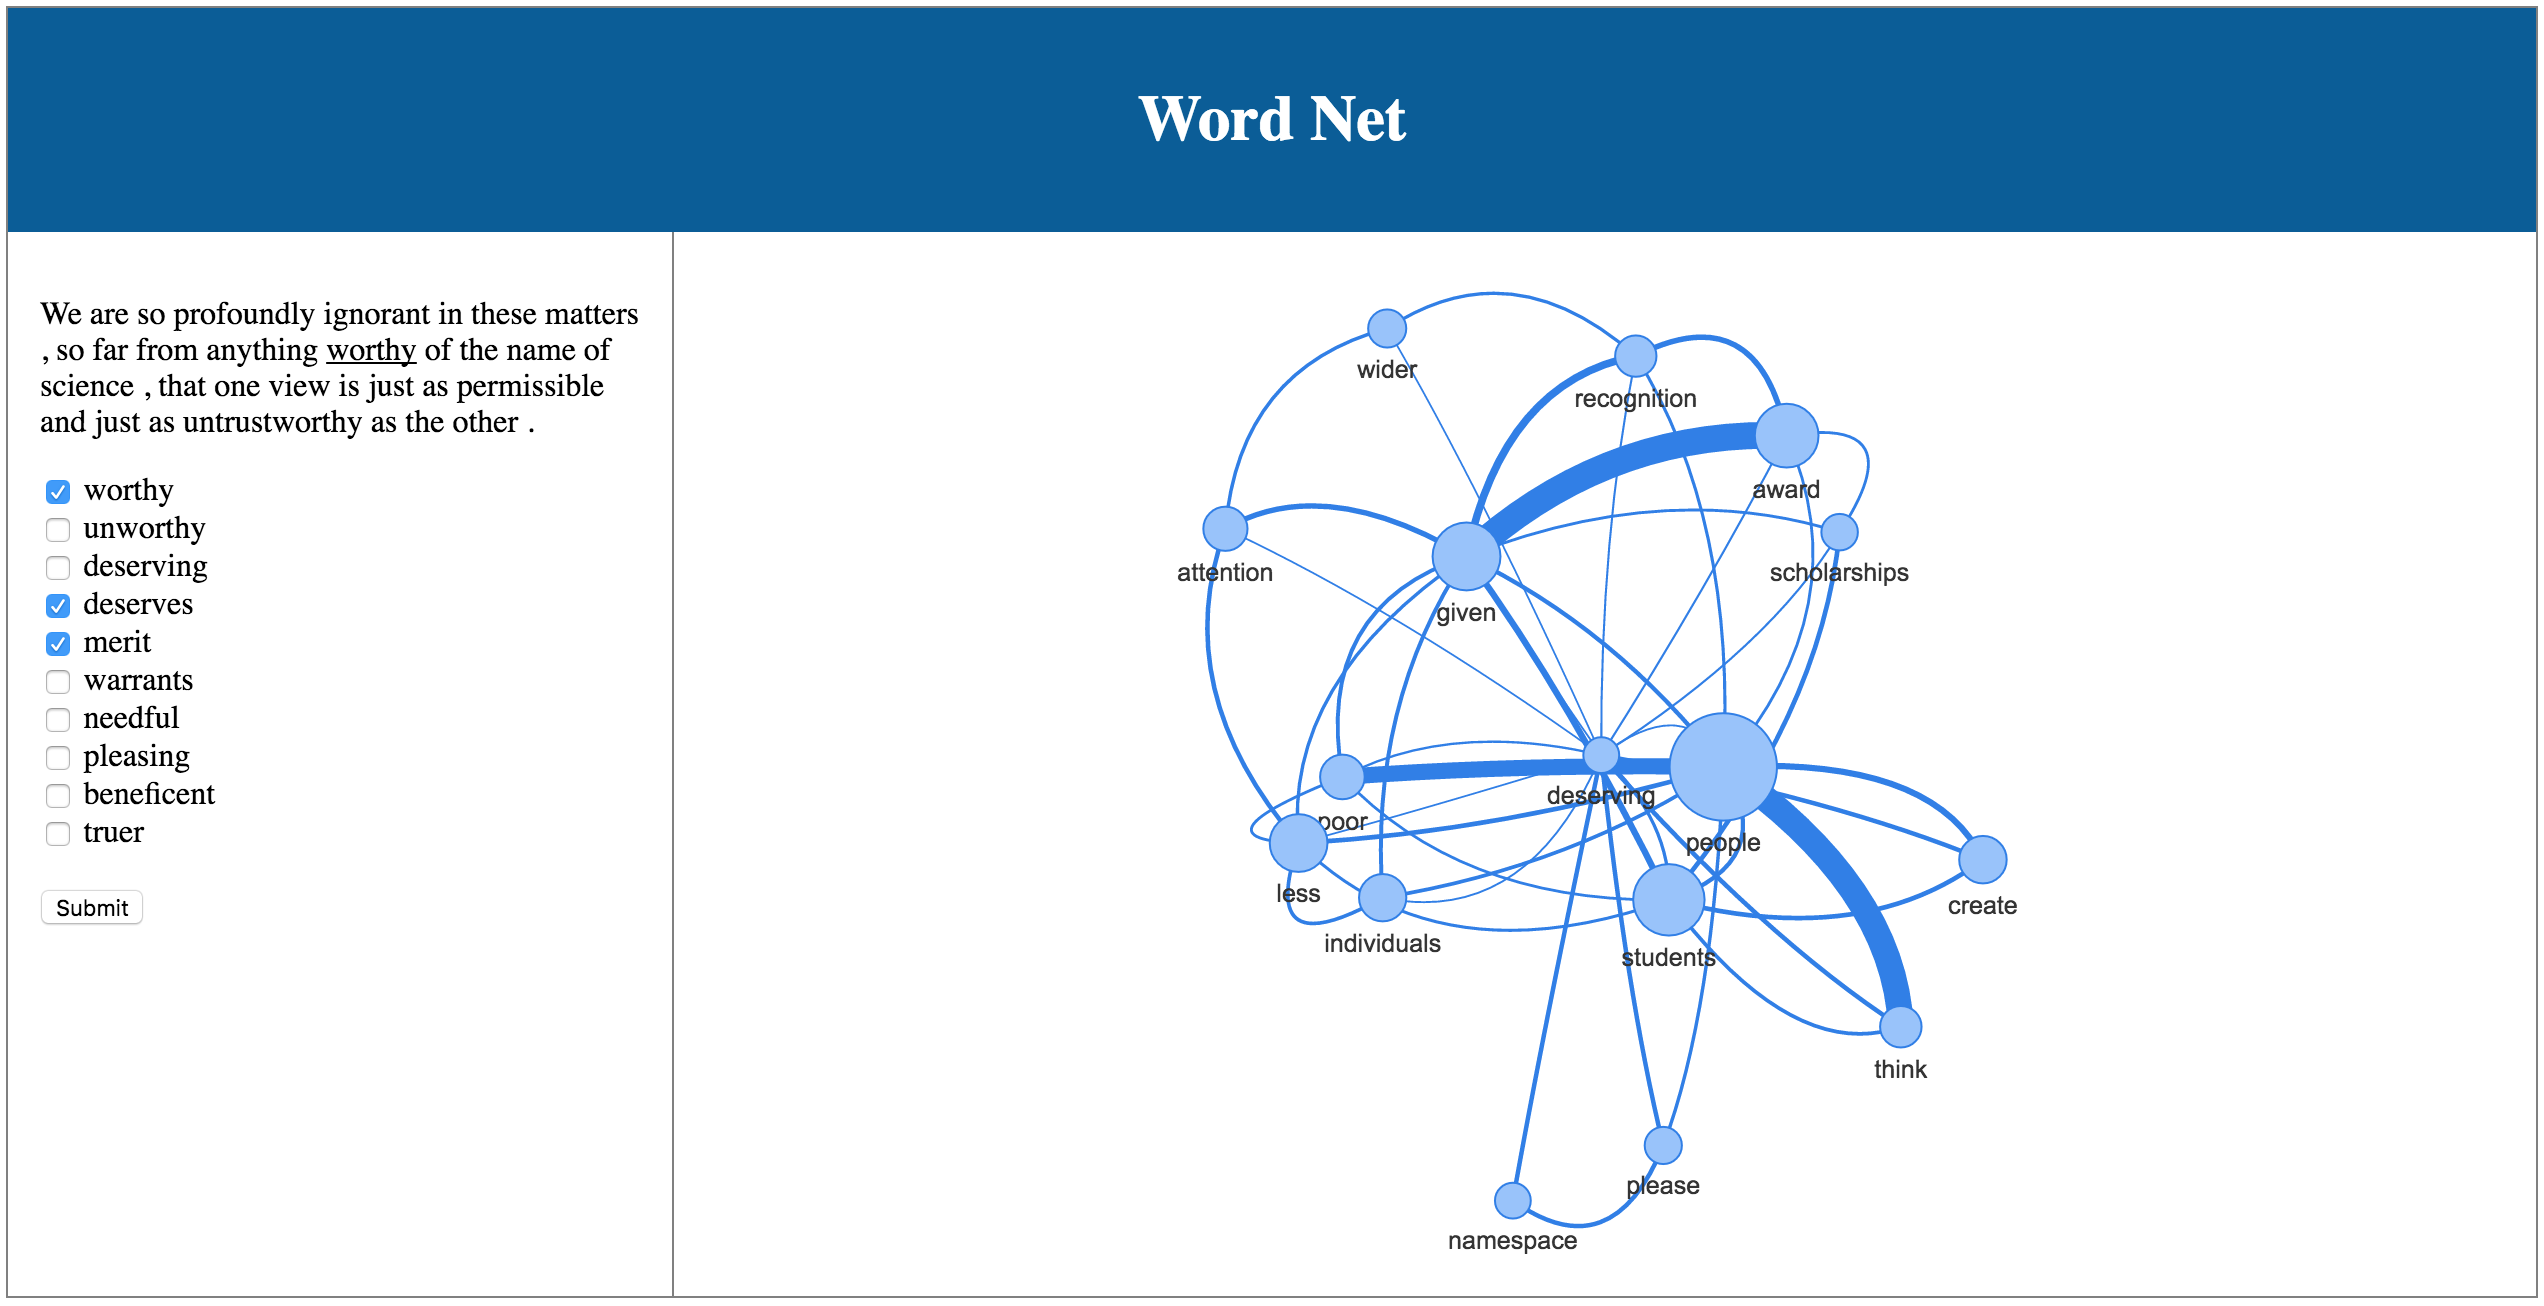
\includegraphics[width=\linewidth]{figure/net_demo_new}
\caption{Visualization of a new word network selected by user}
\label{fig:net_demo_new}
\end{figure}


\subsection{Pipeline design}


The pipeline for our project is very simple, it includes three parts, and we describe more implementation details in Section \ref{sec:impl}.

\begin{enumerate}
	\item Back-end: to generate data. We use python to implement it.
	
	\item Web framework: to exchange data between back-end and front-end by post and request, and to deploy it online and control the routing. We use flask to implement it.
	
	\item Front-end: the user interface. We use Javascript + HTML + CSS to implement it.
\end{enumerate}
